\documentclass[a4paper,12pt]{article} % тип документа
\usepackage[margin=1in]{geometry} % Поля

%  Русский язык
\usepackage[warn]{mathtext}
\usepackage[T2A]{fontenc}			% кодировка
\usepackage[utf8]{inputenc}			% кодировка исходного текста
\usepackage[english,russian]{babel}	% локализация и переносы
% Математика
\usepackage{amsmath,amsfonts,amssymb,amsthm,mathtools} 
\usepackage{wasysym}
%%%
\usepackage{graphicx}

\usepackage{gensymb} % знак градуса
\usepackage{enumitem} % изменить список enumerate

%%%% Римские цифры
\renewcommand{\thesection}{\Roman{section}.} 
\renewcommand{\thesubsection}{\roman{subsection}.}


\begin{document}
%титул
\hrule 	
\medskip
\begin{raggedright}
{\large \textbf{Отчёт по работе 2.1.6}}
\\
\medskip
{\Large Эффект Джоуля-Томсона} 
\\
\medskip
{\large Карташов Константин Б04-005}
\medskip
\hrule
\medskip
\end{raggedright}


\section{Аннотация}

\subsection{Цель работы}

\begin{enumerate}
\item Измерение эффекта Джоуля-Томсона для углекислого газа. Измерение изменения температуры газа при протекании через малопроницаемую перегородку при разных значениях давления и температуры.
\item Вычисление по результатам опытов коэффициентов Ван-дер-Ваальса <<a>> и <<b>>.
\end{enumerate}


\medskip\hrule\medskip

\section{Теоретическая часть}

\paragraph{}
Эффектом Джоуля–Томсона называется изменение температуры газа, медленно протекающего  из области высокого в область низкого давления в условиях хорошей тепловой изоляции. В разреженных газах, которые приближаются по своим свойствам к идеальному  газу, при таком течении температура газа не меняется. Эффект Джоуля–Томсона демонстрирует отличие исследуемого газа от идеального.

\paragraph{}
Эффект Джоуля-Томсона характеризуется коэффициентом Джоуля-Томсона, показывающего отношение изменения температуры газа при расширении к изменению давления. В работе используется приближенная формула нахождения коэффициента Джоуля–Томсона (формула \ref{vander}) для газа Ван-дер-Ваальса, уравненим состояния которого является формула 2, в котором $V$ - молярный объём, $a$ и $b$ - коэффициенты Ван-дер-Ваальса. 

\begin{equation}\label{vander}
\mu_\text{д-т} = \frac{\Delta T}{\Delta P} \approx \frac{\frac{2a}{RT} - b}{C_p}.
\end{equation}

\begin{equation}\label{gas}
\left( P + \frac{a}{V^2} \right) \left( V - b \right) = RT
\end{equation}


\medskip\hrule\medskip

\section{Экспериментальная часть}

\subsection{Устройство экспериментальной установки}


\begin{figure}[h]
\centering
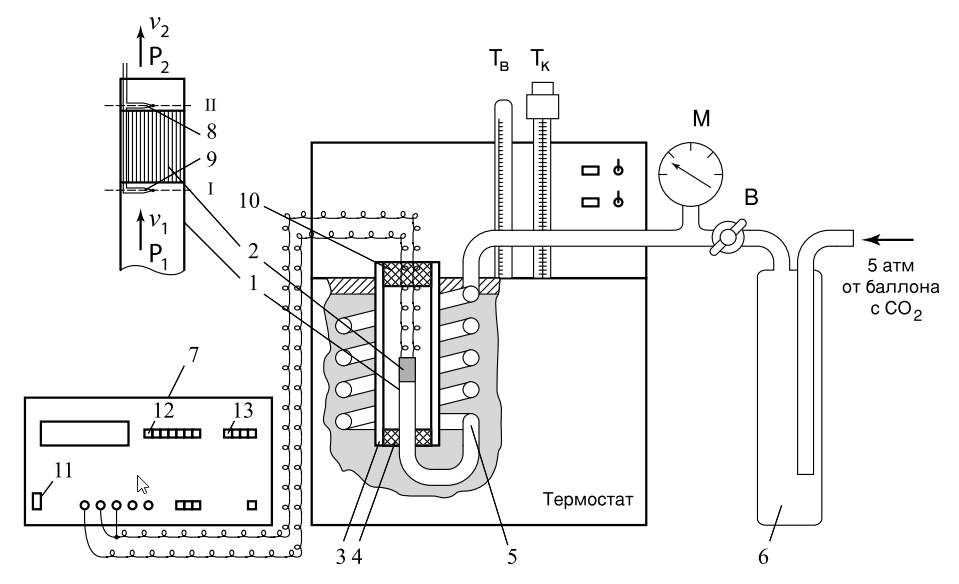
\includegraphics[scale=0.4]{setup.jpg}
\caption{Схема экспериментальной установки.}
\label{fig:setup}
\end{figure}


Обозначения на рисунке \ref{fig:setup}:\\
1 -- Трубка\\
2 -- Пористая перегородка\\
3 -- Трубка Дьюара\\
4 -- Кольцо для теплоизоляции\\
5 -- Змеевик\\
6 -- Балластный баллон\\
7 -- Цифровой вольтметр, к которому подключены медные проволоки\\
8, 9 -- Спаи соединённые константановой проволокой\\
10 -- Пробка из пенопласта для теплоизоляции\\
11 -- Выключатель <<Сеть>>\\
12 -- Кнопка <<АПВ>>\\
13 -- Кнопка <<$U_=$>>\\
В -- Вентиль  для регулировки потока газа\\
М -- Манометр\\



\subsection{Проведение эксперимента}

\begin{enumerate}
\item Убедимся в целостности экспериментальной установки: проверим заполненность термостата, проверим закреплены  ли все электрические приборы и находятся ли они в рабочем состоянии. 
\item  Установим на контактном термометре  $T_\text{К}$ температуру регулирования, близкую к комнатной, и включим термостат.
\item Включим вольтметр в режиме <<АВП>> (автоматический выбор предела). Запишем значение вольтметра при $\Delta P = 0$.
\item Откроем регулирующий вентиль В настолько, чтобы установилось избыточное давление $\Delta P \approx 4 \; \text{атм}$. Через 10-15 минут после подачи давления, когда затухнут переходные процессы, запишем показания вольтметра.
\item При помощи вентиля В уменьшим давление в установке на 0,3-0,5 атм меньше первоначального, после установление давления и разности температур вновь запишем показания манометра и вольтметра.
\item Повторим эти измерения для 5-7 различных значений давления  при комнатной температуре.
\item Закончив измерения при комнатной температуре закроем вентиль В и установим на контактном термометре температуру 30 \degree C.
\item После установления температуры  повторим измерения следуя пунктам 4-6.
\item Увеличим температуру до 50 \degree C и повторим измерения следуя пунктам 7 и 8.
\item Далее перейдём  к обработкам результатов.
\end{enumerate}

\subsection{Обработка результатов}

\paragraph{}
Результаты полученные  после проведения  измерений приведены в приложении. Переведём их в нужный вид. Значения для разницы давления даны в больших делениях манометра, манометр имеет 100 больших делений с одним маленьким делением между ними. На 100 делений манометра приходится 
6 $ \text{кгс} / \text{см}^2 $, 
переведём эти значения в атмосферы ($ 1 \text{дел} \approx 0.058 \text{атм} $).
 Переведём разницу потенциалов на электропаре в разницу температуры для каждого измерения запишем 
 $ \Delta U_i = U_i - U_0 $ ($ i $ - номер измерения). 
 Дальше переведём $ \Delta U $ в $ \Delta T $ по соотношению: 
 $ \Delta T = \alpha \Delta U$,
 где $\alpha$ зависит от значения температуры термостата:
\begin{center} 
 \begin{tabular}{|c||c|c|c|}
 \hline 
 $\tau$, \degree C & 18 & 30 & 50 \\ 
 \hline 
 $\alpha$, мкВ / K & 39,8 & 41,6 & 43,3 \\ 
 \hline 
 \end{tabular}
\end{center} 
 Результаты записаны в таблицах 1, 2 и 3.

%Таблицы с измеренными данными

%%%
\begin{table}
\begin{center}
\begin{tabular}{ |c||c|c|c| } 

 \hline
 N & $\Delta P$, атм & $\tau$, \degree C & $\Delta T$, K \\
 \hline
0 & 0.0 & 18.0 & 0.0 \\
1 & 4.065 & 18.15 & 4.322 \\
2 & 3.717 & 18.23 & 3.894 \\
3 & 3.339 & 18.29 & 3.467 \\
4 & 2.962 & 18.37 & 3.015 \\
5 & 2.671 & 18.45 & 2.663 \\
6 & 1.974 & 18.51 & 1.859 \\
7 & 1.713 & 18.62 & 1.583 \\
 \hline

\end{tabular}
\end{center}
\caption{Обработанные результаты измерения 1}
\end{table}

%%%
\begin{table}
\begin{center}
\begin{tabular}{ |c||c|c|c| } 

 \hline
 N & $\Delta P$, атм & $\tau$, \degree C & $\Delta T$, K \\
 \hline
0 & 0.0 & 30.06 & 0.0 \\
1 & 4.181 & 30.1 & 3.846 \\
2 & 3.862 & 30.08 & 3.462 \\
3 & 3.078 & 30.01 & 2.62 \\
4 & 2.671 & 30.02 & 2.188 \\
5 & 2.584 & 30.0 & 2.115 \\
6 & 2.236 & 30.0 & 1.755 \\
7 & 1.568 & 30.0 & 1.082 \\
 \hline

\end{tabular}
\end{center}
\caption{Обработанные результаты измерения 2}
\end{table}

%%%
\begin{table}
\begin{center}
\begin{tabular}{ |c||c|c|c| } 

 \hline
 N & $\Delta P$, атм & $\tau$, \degree C & $\Delta T$, K \\
 \hline
0 & 0.0 & 50.0 & 0.0 \\
1 & 4.007 & 50.04 & 2.956 \\
2 & 3.775 & 50.04 & 2.656 \\
3 & 3.339 & 50.01 & 2.286 \\
4 & 2.933 & 50.0 & 1.894 \\
5 & 1.945 & 50.0 & 1.016 \\
 \hline

\end{tabular}
\end{center}
\caption{Обработанные результаты измерения 3}
\end{table}

\paragraph{}
Найдём систематические погрешности. Погрешность $ \sigma_{\Delta P} = 0.5 \text{ дел} = 0.03 \text{ атм}$. Погрешность $\sigma{\Delta U} = 0.001 \text{ мкВ} $ из чего находим погрешность $\sigma_{\Delta T}$, она зависит от температуры так как при разных температурах мы используем разные коэффициент для перевода $\Delta U$ в $\Delta T$ при различных температурах термостата, но так как значения $\alpha$ отличаются друг от друго не более чем на 5\% возьмём $\alpha = 39.8 \text{ мкВ/К}$, получаем $\sigma_{\Delta T} = 0.05$ K.



\paragraph{}
По получившимся значениям для $\Delta P$ и $\Delta T$ построим график зависимости $\Delta T \left( \Delta P \right)$. И пользуясь методом наименьших квадратов найдём аппроксимирующую прямую. Метод наименьших квадратов для построения прямой $ y = A + B x $:
\[
B = \frac{\langle xy \rangle - \langle x \rangle \langle y \rangle}{\langle x^2 \rangle - \langle x \rangle ^ 2}, \;\;
A = \langle y \rangle - B \langle x \rangle .
\]
Найдём погрешности коэффициентов $a$ и $b$ по формулам:
\[
\sigma_B \approx \frac{1}{\sqrt{N}}\sqrt{\frac{\langle y^2 \rangle - \langle y \rangle ^ 2}{\langle x^2 \rangle - \langle x \rangle ^ 2} - B^2}, \;\;
\sigma_A = \sigma_B \sqrt{\langle x^2 \rangle - \langle x \rangle ^ 2}.
\]
Подставим значения из таблиц 1, 2 и 3: $\Delta P$ вместо $x$ и $\Delta U$ вместо $y$, полученные значения запишем в таблицу 4:

\begin{table}[h]
\begin{center}
\begin{tabular}{|c||c|c|c|}
\hline 
 & $\tau = 18\text{\degree C}$ & $\tau = 30\text{\degree C}$ & $\tau = 50\text{\degree C}$ \\ 
\hline 
$B$, K/атм & 1,167 & 1,06 & 0,93 \\ 
\hline 
$\sigma_B$, К/атм & 0,006 & 0,01 & 0,02 \\ 
\hline 
$A$, К & -0,437 & -0,61 & -0,80 \\ 
\hline 
$\sigma_A$, К & 0,008 & 0,01 & 0,01 \\ 
\hline 
\end{tabular} 
\end{center}
\caption{Значения полученные для A и B}
\end{table}

\paragraph{}
Покажем точки из таблиц 1, 2, 3 и соответивующие им прямые с коэффициентами из таблицы 4 на графике (Рис 2).	Получим значенния для коэффиуиента Джоуля-Томсона:
\[
\mu_\text{Д-Т} = \frac{\Delta T}{\Delta P} = \frac{A + B \Delta P}{\Delta P} = B + \frac{A}{\Delta P}
\]
Погрешность для $\frac{A}{\Delta P}$: 
\[
\sigma_{A'} = \frac{A}{\Delta P} \sqrt{\left(\frac{\sigma_A}{A}\right)^2 + \left(\frac{\sigma_{\Delta P}}{\Delta P}\right)^2}. 
\]
Диапазон измерений: $ 1,5\text{ атм} < \Delta P < 4,5 \text{ атм} $, значит:
\[
\max{\sigma_{A'}} = \frac{A}{4,5 \text{ атм}} \sqrt{\left(\frac{\sigma_A}{A}\right)^2 + \left(\frac{\sigma_{\Delta P}}{\Delta P}\right)^2}. 
\]
Теперь посчитаем константу Джоуля-Томсона для трёх значений температуры в определённом ранее диапазоне:

 
\[
\tau = 18 \text{°C}: \; \mu_\text{Д-Т} = 1,167 \pm 0,006 \text{ К/атм} - \frac{0,437 \text{ К}}{\Delta P} \pm 0,002  \text{ К/атм}
\]

\[
\tau = 30 \text{°C} : \; \mu_\text{Д-Т} = 1,06 \pm 0,01 \text{ К/атм} - \frac{0,61 \text{ К}}{\Delta P} \pm 0,002  \text{ К/атм}
\]

\[
\tau = 50 \text{°C}: \; \mu_\text{Д-Т} = 0,93 \pm 0,02 \text{ К/атм} - \frac{0,80 \text{ К}}{\Delta P} \pm 0,005  \text{ К/атм}
\]

\paragraph{}
Константы Джоуля-Томсона получились получились зависимыми от разницы давления, поэтому для подсчёта коэффициэнтов a и b из уравнения Ван-дер-Ваальса используем усреднённое значение коэффициентов джоуля полученные нами для диапазона давленя, расчитанные по формуле:

\[
\bar{\mu} = \frac{
	\mu_\text{Д-Т}\left( 1,5 \text{ атм} \right) + \mu_\text{Д-Т}\left( 4,5 \text{ атм} \right)}{2}, \;  \sigma_{\bar{\mu}} = \mu_\text{Д-Т}\left( 1,5 \text{ атм} \right) - \bar{\mu}.
\]

\begin{table}[h]	
\begin{center}
\begin{tabular}{|c|c|}
\hline 
$\tau$,\degree C & $\bar{\mu} \pm \sigma_{\bar{\mu}}$, К/атм \\ 
\hline 
18 & $1,0 \pm 0,2$  \\ 
\hline 
30 & $0,8 \pm 0,3$ \\ 
\hline 
50 & $0,6 \pm  0,4$\\ 
\hline 
\end{tabular} 
\end{center}
\caption{Рассчитанные коэффициенты Джоуля-Томсона}
\end{table}


\begin{figure}
\begin{center}
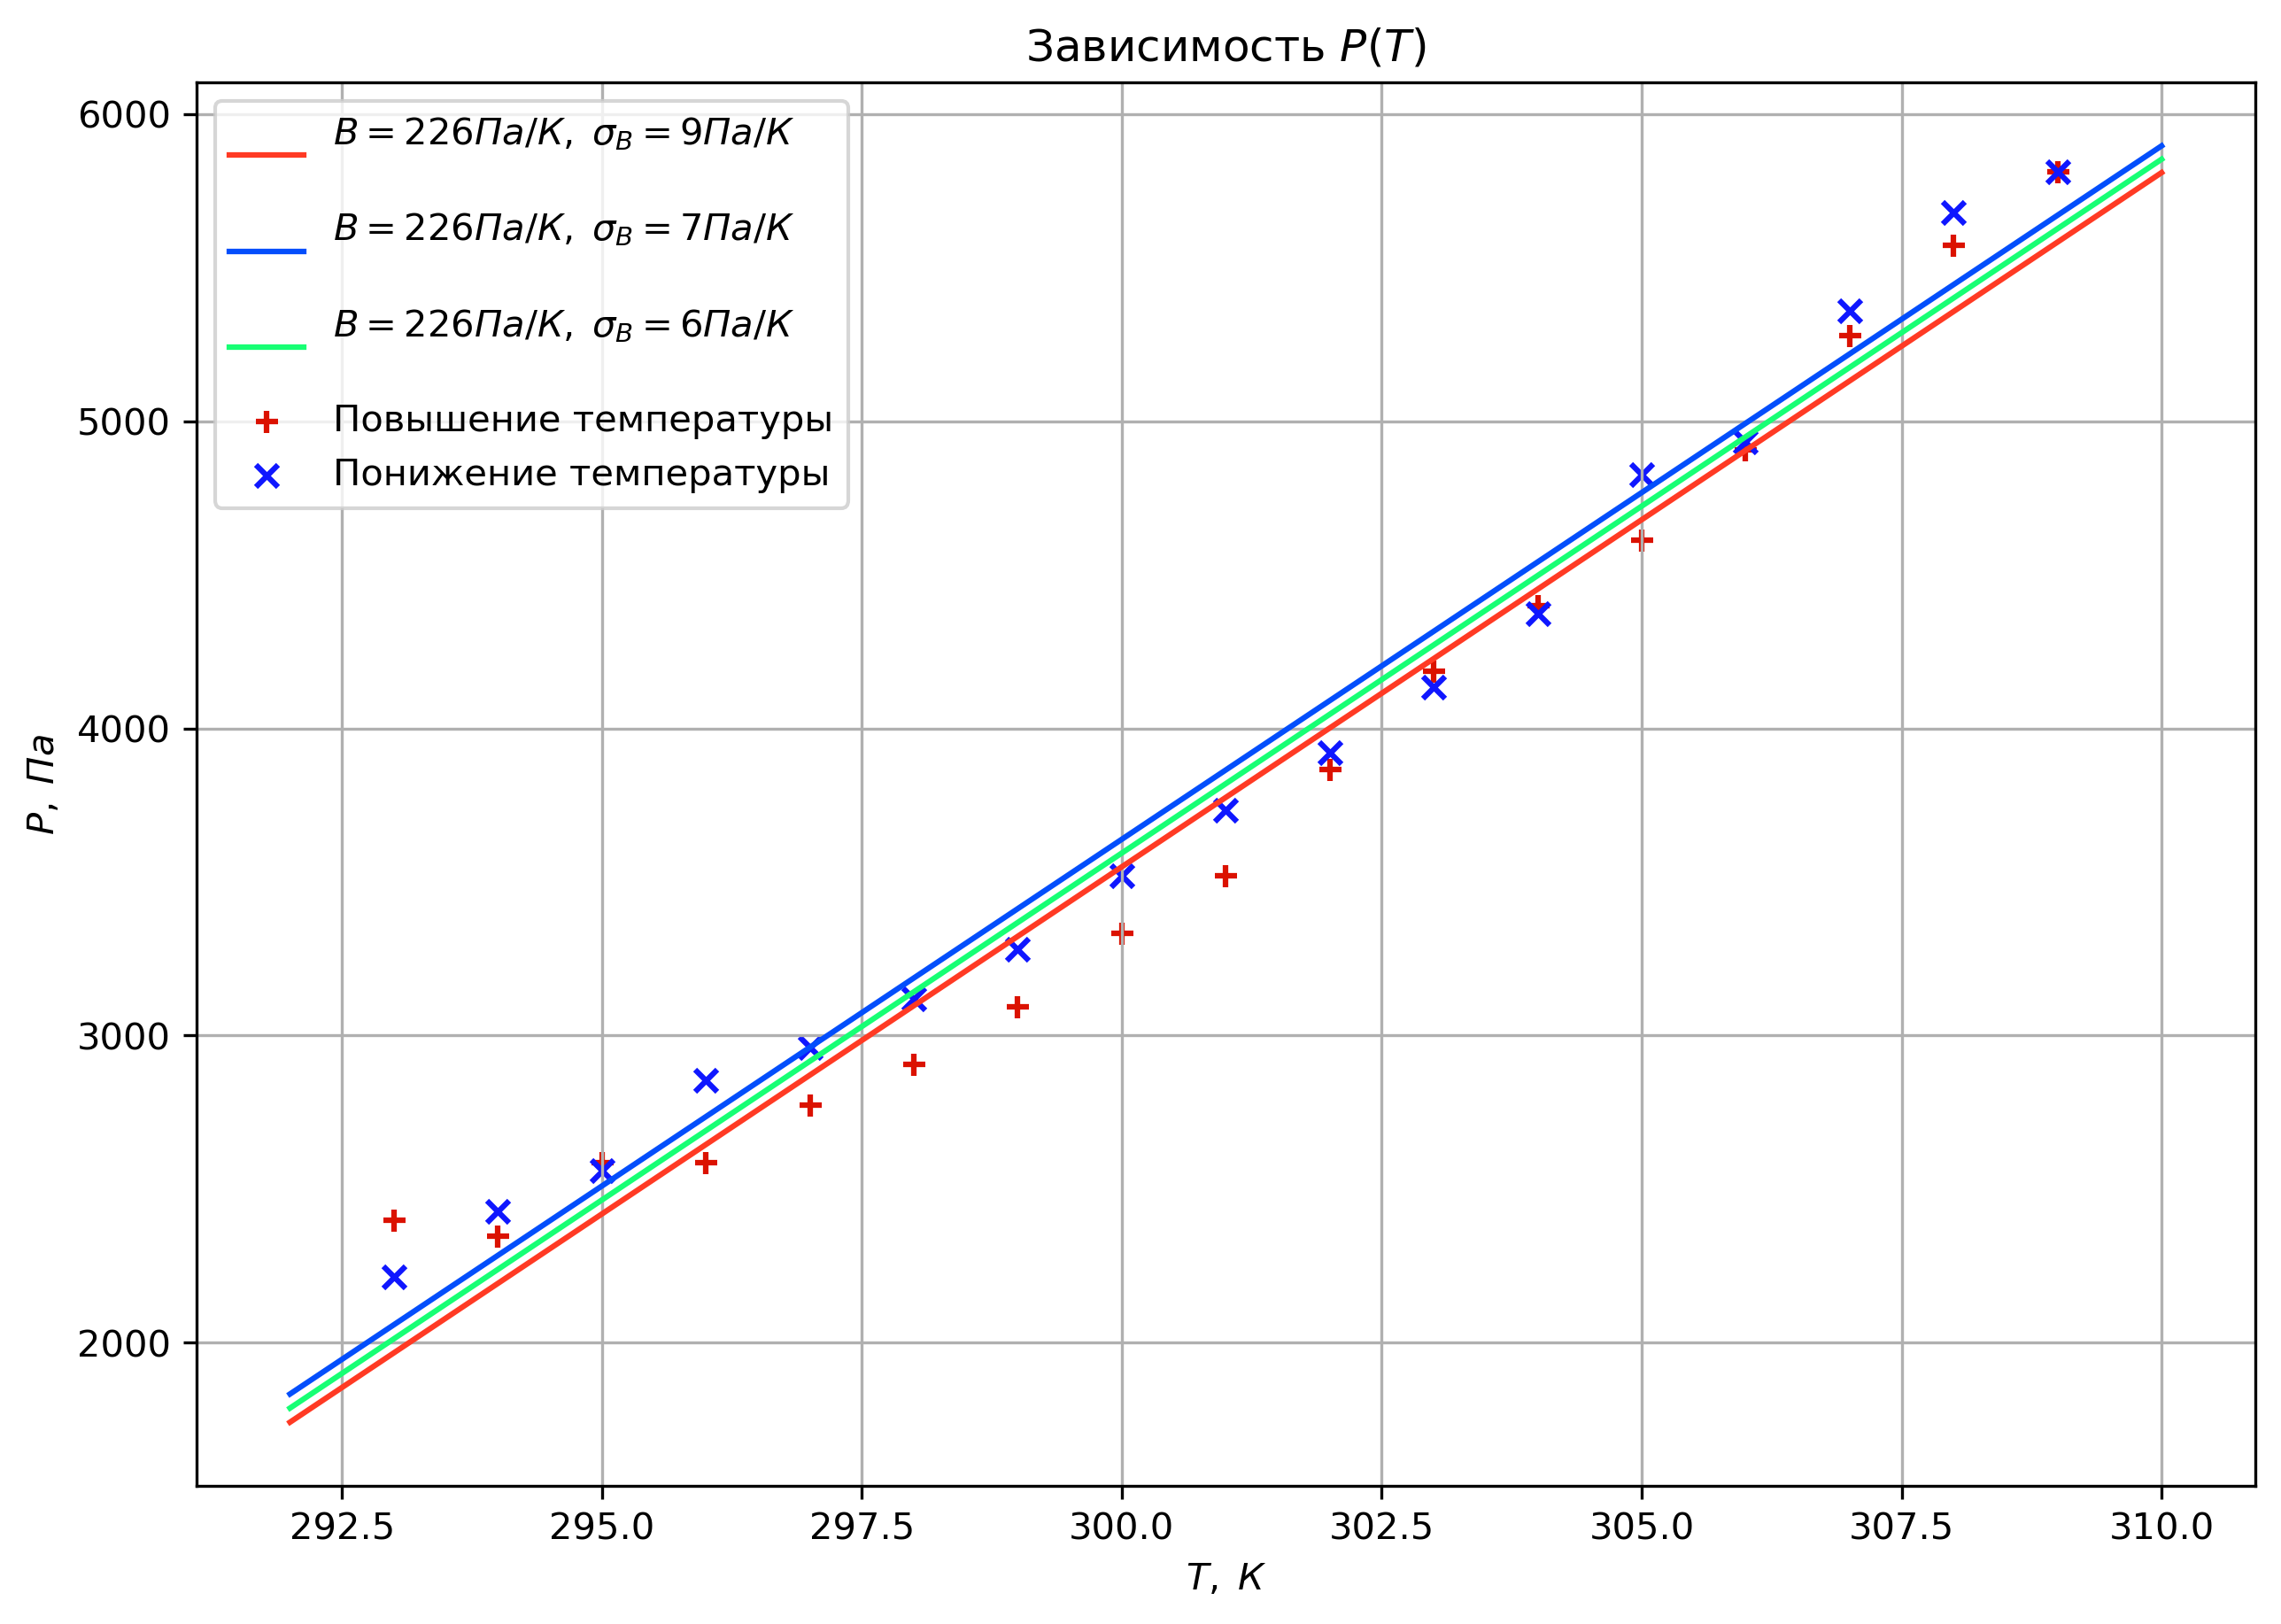
\includegraphics[scale=1]{graph1.jpg}
\end{center}
\caption{График данных}
\end{figure}

\paragraph{}
На основе полученных значений для коэффициэнта Джоуля-Томсона рассчитаем коэффициэнты Ван-дер-Ваальса по формуле \ref{vander}. Для этого возьмём два значения $\mu_1$ и $\mu_2$ и решим систему из двух уравнений:

\[
\begin{cases} 
\mu_1 = \frac{\frac{2a}{R T_1} - b}{C_p} \\
\mu_2 = \frac{\frac{2a}{R T_2} - b}{C_p}
\end{cases}
\Leftrightarrow
\begin{cases}
b = \frac{C_p \left(T_1 \mu_1 - T_2 \mu_2 \right)}{T_2 - T_1} \\
a = \frac{2 C_p R \left( \mu_1 - \mu_2 \right) }{2 \left( 1/T_1 + 1/T_2 \right)}

\end{cases}
\]


Погрешности для a и b найдём пользуясь формулами погрешностей для сумм и произведений для полученных выражений. Заметим, что погрешности $\mu_1$ и $\mu_2$ намного больше погрешностей для значений температуры, поэтому получим погрешности:

\[
\sigma_b = b \frac{\sqrt{T_1^2 \sigma_{\mu_1}^2 + 
T_2^2 \sigma_{\mu_2}^2}}{T_1 \mu_1 - T_2 \mu_2}
\]

\[
\sigma_a = a \frac{\sqrt{\sigma_{\mu_1}^2 + \sigma_{\mu_2}^2}}{\mu_1 - \mu_2}
\]

Подставим в эти формулы значения коэффициента Джоуля-Томсона для разных значений температуры, результат запишем в таблицу 6. Видим, что погрешности получились зачастую больше самих значений коэффициентов, что делает их непригодными для дальнейших рассчётов.

\begin{table}
\begin{center}
\begin{tabular}{|c|c|c|c|}
\hline 
$T_1$ \degree C & 18 & 30 & 50 \\ 
\hline 
$T_2$ \degree C & 30 & 50 & 18 \\ 
\hline \hline 
$a$ & 3592 & 7410 & -3784 \\ 
\hline 
$\sigma_a$ & 2335 & 3705 & 4730 \\ 
\hline 
$b$ & 117 & 88 & 70 \\ 
\hline 
$\sigma_b$ & 261 & 128 & 229 \\ 
\hline 
\end{tabular} 
\end{center}
\caption{Значения коэффициентов a и b}
\end{table}

Погрешность большая, чем сам значения говорит о полной непригодности этих данных для какх либо рассчётов.

\medskip\hrule\medskip

\section{Выводы}
\paragraph{}
В ходе эксперимента был измерен эффект Джоуля-Томсона. Значения коэффициэнтов Джоуля-Томсна полученные в ходе лабораторной работы (таблица 4) сильно отличаются от табличных данных при $\Delta P = 1$, однако без слагаемого $A / \Delta P$ значения очень близки к табличным (Значение для $\tau = 18 \degree C$ лежит между табличными значениями для температуры 0 \degree C и 20 \degree C, для $\tau = 30 \degree C$  между 20 \degree C и 40 \degree C, аналогично для $\tau = 50 \degree C$). Это может свидетельствовать о неучтённых внешних условиях, смещающих значение коэффициента Ван-дер-Ваальса. 

\paragraph{}
Значения для коэффициентов газа Ван-дер-Ваальса имеюст слишком большую погрешность из-за неточности в измерении коэффициэнта Джоуля-Томсона. Эти расхождения могут быть объяснены ошибками в проведении эксперимента. 
\medskip\hrule\medskip


\end{document}


